% A4縦・1段組の学習用（教科書風）
\documentclass[paper=a4,fleqn]{jlreq}
\special{papersize=\the\paperwidth,\the\paperheight}

\usepackage[margin=20truemm]{geometry}
\usepackage[dvipdfmx]{graphicx}
\usepackage{amsmath,amssymb}
\usepackage{tikz}
\usepackage{pgfplots}
\usepackage{etoolbox}
\usepackage{needspace}
\pgfplotsset{compat=1.18}
\usetikzlibrary{arrows.meta,calc,angles,quotes}
\usepackage{bm}

% 公式・キーポイントを目立たせるコマンド
\newcommand{\formula}[1]{%
  \vspace{4pt}%
  \begin{center}{\large\bfseries\boldmath\(\displaystyle #1\)}\end{center}%
  \vspace{4pt}%
}

% If there is not enough space left, start the section on the next page.
\preto{\section}{\needspace{0.35\textheight}}
\preto{\subsection}{\needspace{0.32\textheight}}

\ModifyHeading{section}{
  lines=1,
  before_space=14pt,
  after_space=6pt
}

\ModifyHeading{subsection}{
  lines=1,
  before_space=10pt,
  after_space=4pt
}

\title{関数と方程式}
\author{}
\date{}

\makeatletter
\renewcommand{\maketitle}{%
  \begin{center}
    {\large\bfseries \@title\par}
  \end{center}
  \vspace{4pt}
}
\makeatother

\begin{document}
\maketitle

%==========================================================
\section{関数とは何か}
%==========================================================

\subsection{「入力 → 出力」のルール}

\textbf{関数}とは，ある数（入力）を決めると，それに対応する数（出力）が\textbf{1つだけ}決まる対応規則のことである。
難しく考えなくてよい――「\(x\) を入れると \(y\) が1つ出てくる計算機」のようなものだと思えばよい。

\formula{x \;\xrightarrow{\;\text{ルール}\;}\; y}

この対応規則を記号で書くと \(y = f(x)\) となる。
\(f(x)\) は「\(x\) を入力したときの出力」を表す。

\vspace{4pt}
\textbf{例：}
\begin{itemize}
  \item 実数 \(x\) を2倍する対応：\(f(x) = 2x\)
  \item 実数 \(x\) を2乗して1を加える対応：\(f(x) = x^2 + 1\)
  \item 実数 \(x\) に対して \(3x - 5\) を対応させる規則：\(f(x) = 3x - 5\)
\end{itemize}

\subsection{\(f(x)\) の書き方}

関数は \(f(x) = \text{式}\) の形で定義する。

\begin{itemize}
  \item \(f(x) = 2x\) \quad …\(x\) を2倍した値
  \item \(f(x) = x^2 + 1\) \quad …\(x\) を2乗して1を加えた値
  \item \(f(x) = 3x - 5\) \quad …\(x\) を3倍して5を引いた値
\end{itemize}

\(x\) に具体的な数を代入すれば，その点での関数値が求まる。

\[
  f(x) = 2x + 1 \quad\text{のとき} \quad
  f(3) = 2 \times 3 + 1 = 7,\quad
  f(0) = 1,\quad
  f(-2) = -3
\]

\subsection{表と対応表で見る関数}

関数は「対応表」にすると，入力と出力の関係が直感的に見える。

\textbf{例：} \(f(x)=2x+1\)

\begin{center}
\renewcommand{\arraystretch}{1.5}
\begin{tabular}{c|ccccc}
\hline
\(x\) & -2 & -1 & 0 & 1 & 2 \\
\hline
\(f(x)\) & -3 & -1 & 1 & 3 & 5 \\
\hline
\end{tabular}
\end{center}

この表から，\(x\) を1ずつ増やすと \(f(x)\) が2ずつ増えることがわかる。
式・表・グラフは同じ関数を別の形で表したものである。

\needspace{0.42\textheight}
\subsection{変数と定数}

式の中には2種類の文字がある。

\begin{itemize}
  \item \textbf{変数}（variable）：値が変わりうる文字。主に \(x, y, t\) など。
  \item \textbf{定数}（constant）：値が固定された数や文字。主に \(a, b, c, v, g\) など。
\end{itemize}

\(f(x)=ax+b\) では \(x\) が変数，\(a,b\) が定数である。

\subsection{グラフで見る関数}

関数 \(y = f(x)\) をグラフにすると，\textbf{すべての \(x\) の値に対応する点を連続的に結んだ曲線（または直線）}が得られる。

\begin{center}
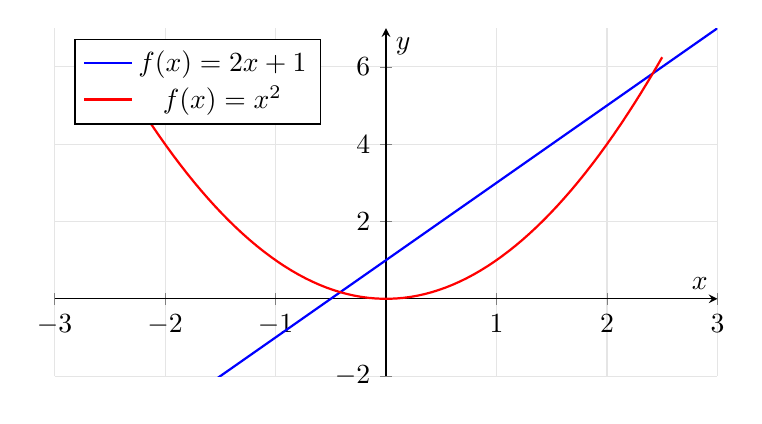
\begin{tikzpicture}
  \begin{axis}[
    width=10cm, height=6cm,
    axis lines=middle,
    xmin=-3, xmax=3, ymin=-2, ymax=7,
    xlabel={$x$}, ylabel={$y$},
    grid=both, grid style={gray!20},
    legend pos=north west
  ]
    \addplot[blue, thick, domain=-3:3, samples=80] {2*x+1};
    \addlegendentry{$f(x)=2x+1$}
    \addplot[red, thick, domain=-2.5:2.5, samples=80] {x^2};
    \addlegendentry{$f(x)=x^2$}
  \end{axis}
\end{tikzpicture}
\end{center}

グラフを見れば，\(x\) を変えると \(y\) がどう変わるかが\textbf{一目で}わかる。これが関数のもつ強みである。

\subsection{確認問題}
\begin{enumerate}
  \item \(f(x) = 3x - 2\) のとき，\(f(0),\ f(2),\ f(-1)\) を求めよ。
  \item \(f(x) = x^2 + x - 1\) のとき，\(f(0),\ f(2),\ f(-3)\) を求めよ。
  \item \(f(x) = x^2 - 3\) のとき，\(f(3)\) を求めよ。
\end{enumerate}

\newpage
%==========================================================
\section{関数と方程式の違い}
%==========================================================

\subsection{「動く線」と「止まった点」}

関数と方程式は，見た目が似ていることがあるが，\textbf{問いかけ方がまったく異なる}。

\vspace{8pt}
\begin{center}
\renewcommand{\arraystretch}{1.6}
\begin{tabular}{p{4cm}|p{5cm}|p{4.5cm}}
\hline
& \textbf{関数} & \textbf{方程式} \\
\hline
意味 & \(x\) が決まると \(y\) が決まる対応ルール & 特定の \(x\) の値を求める等式 \\
目的 & すべての \(x\) に対する \(y\) の変化を表す & 条件を満たす \(x\)（解）を探す \\
答えのイメージ & \textbf{線（グラフ）} & \textbf{点（値）} \\
例 & \(y = 2x + 1\)（すべての \(x\) で成立） & \(2x + 1 = 7\)（\(x = 3\) のみ） \\
\hline
\end{tabular}
\end{center}

\vspace{8pt}
まとめると：

\vspace{4pt}
\begin{center}
{\large\bfseries\boldmath
  \textbf{方程式}：特定の \(x\) の値（解）を求める等式\quad $\rightarrow$\quad 「止まった点」\\[6pt]
  \textbf{関数}：\(x\) に応じて \(y\) が決まる対応規則\quad $\rightarrow$\quad 「動く線」
}
\end{center}
\vspace{4pt}

\subsection{具体例で比べる}

\(y = 2x + 1\) という式は，2つの見方で用いることができる。

\begin{itemize}
  \item \textbf{関数として見る}：任意の \(x\) に対して \(y\) が定まる。グラフは直線である。
  \item \textbf{方程式として用いる}：「\(y = 7\) となる \(x\) は何か」→ \(2x + 1 = 7\) を解くと \(x = 3\)。
\end{itemize}

\begin{center}
\begin{tikzpicture}
  \begin{axis}[
    width=9cm, height=6cm,
    axis lines=middle,
    xmin=-2, xmax=5, ymin=-2, ymax=10,
    xlabel={$x$}, ylabel={$y$},
    grid=both, grid style={gray!20}
  ]
    \addplot[blue, thick, domain=-2:5] {2*x+1};
    \addplot[only marks, mark=*, mark size=3pt, red] coordinates {(3,7)};
    \draw[dashed, red] (axis cs:3,0) -- (axis cs:3,7) -- (axis cs:0,7);
    \node[red, right] at (axis cs:3.1,7) {$(3,\,7)$：方程式の解};
    \node[blue, right] at (axis cs:3.5,2.5) {$y=2x+1$：関数};
  \end{axis}
\end{tikzpicture}
\end{center}

関数（青い直線全体）の中の1点（赤い点）が，方程式の解である。

\newpage
%==========================================================
\section{直線の方程式}
%==========================================================

\subsection{直線の方程式の形}

直線は以下の形で表される。

\formula{y = ax + b}

\begin{itemize}
  \item \(a\)：\textbf{傾き}（slope）。\(x\) が1増えると \(y\) が \(a\) 増える。
  \item \(b\)：\textbf{切片}（intercept）。\(x = 0\) のときの \(y\) の値（\(y\) 軸との交点）。
\end{itemize}

\subsection{傾きの意味}

\formula{a = \dfrac{y\text{ の増加量}}{x\text{ の増加量}} = \dfrac{\Delta y}{\Delta x}}

\begin{center}
\begin{tikzpicture}[scale=0.9]
  \draw[->] (-0.5,0)--(5,0) node[right] {$x$};
  \draw[->] (0,-0.5)--(0,4.5) node[above] {$y$};
  \draw[blue, thick] (-0.2,0.4)--(4.5,3.5);
  \coordinate (P) at (1,1.2);
  \coordinate (Q) at (3.5,3.05);
  \coordinate (R) at (3.5,1.2);
  \draw[dashed] (P)--(R)--(Q);
  \draw[<->, thick, gray] (1,0.9)--(3.5,0.9) node[midway, below] {$\Delta x$};
  \draw[<->, thick, gray] (3.8,1.2)--(3.8,3.05) node[midway, right] {$\Delta y$};
  \fill (P) circle (2pt);
  \fill (Q) circle (2pt);
\end{tikzpicture}
\end{center}

\subsection{2点から直線を求める}

2点 \((x_1, y_1),\ (x_2, y_2)\) を通る直線の方程式：

\formula{\text{傾き} \; a = \dfrac{y_2 - y_1}{x_2 - x_1} \qquad \text{方程式} \; y - y_1 = a(x - x_1)}

\textbf{例：} 点 \((1, 3)\) と \((3, 7)\) を通る直線

\[
  a = \frac{7-3}{3-1} = 2, \quad
  y - 3 = 2(x-1) \quad \Rightarrow \quad y = 2x + 1
\]

\subsection{グラフ例}

\begin{center}
\begin{tikzpicture}
  \begin{axis}[
    width=10cm, height=6cm,
    axis lines=middle,
    xmin=-3, xmax=3, ymin=-5, ymax=7,
    xlabel={$x$}, ylabel={$y$},
    grid=both, grid style={gray!20},
    legend pos=north west
  ]
    \addplot[blue, thick, domain=-3:3] {2*x+1};
    \addlegendentry{$y=2x+1$（傾き正）}
    \addplot[red, thick, domain=-3:3] {-x+2};
    \addlegendentry{$y=-x+2$（傾き負）}
    \addplot[green!60!black, thick, domain=-3:3] {3};
    \addlegendentry{$y=3$（水平線）}
  \end{axis}
\end{tikzpicture}
\end{center}

\subsection{確認問題}
\begin{enumerate}
  \item 傾き \(3\)，切片 \(-1\) の直線の方程式を書け。
  \item 点 \((2, 5)\) と \((4, 9)\) を通る直線の方程式を求めよ。
  \item \(y = -2x + 4\) で，\(y = 0\) になる \(x\)（\(x\) 切片）を求めよ。
\end{enumerate}

\newpage
%==========================================================
\section{放物線の方程式}
%==========================================================

\subsection{放物線とは}

\textbf{放物線}（parabola）は，次の式で表される曲線である。

\formula{y = ax^2 + bx + c \quad (a \neq 0)}

\begin{itemize}
  \item \(\bm{a > 0}\) のとき：\textbf{下に凸}（開いた口が上向き）
  \item \(\bm{a < 0}\) のとき：\textbf{上に凸}（開いた口が下向き）
  \item \(|a|\) が大きいほど，細く急な曲線になる
\end{itemize}

\subsection{頂点と軸}

\(y = a(x - p)^2 + q\) の形（\textbf{頂点形式}）に変形すると，頂点や軸が直接読み取れる。

\begin{center}
{\large\bfseries\boldmath
  \textbf{頂点}：\((p,\, q)\) \qquad \textbf{軸}：\(x = p\)（左右対称の縦線）
}
\end{center}

\textbf{例：} \(y = x^2 - 4x + 5 = (x-2)^2 + 1\) → 頂点 \((2, 1)\)，軸 \(x = 2\)

\subsection{平方完成}

一般形から頂点形式への変形を\textbf{平方完成}という。

\begin{align*}
  y &= x^2 - 6x + 11 \\
    &= (x^2 - 6x + 9) - 9 + 11 \\
    &= (x - 3)^2 + 2
\end{align*}

→ 頂点 \((3, 2)\)，軸 \(x = 3\)，下に凸。

\subsection{グラフ例}

\begin{center}
\begin{tikzpicture}
  \begin{axis}[
    width=10cm, height=7cm,
    axis lines=middle,
    xmin=-3, xmax=5, ymin=-3, ymax=9,
    xlabel={$x$}, ylabel={$y$},
    grid=both, grid style={gray!20},
    legend pos=north west
  ]
    \addplot[blue, thick, domain=-2:4, samples=80] {(x-1)^2 - 2};
    \addlegendentry{$y=(x-1)^2-2$（頂点$(1,-2)$）}
    \addplot[red, thick, domain=-1.5:3.5, samples=80] {-(x-1)^2 + 4};
    \addlegendentry{$y=-(x-1)^2+4$（頂点$(1,4)$）}
    \addplot[only marks, mark=*, mark size=2.5pt, blue] coordinates {(1,-2)};
    \addplot[only marks, mark=*, mark size=2.5pt, red] coordinates {(1,4)};
  \end{axis}
\end{tikzpicture}
\end{center}

\subsection{放物線の読み取り練習}

\(y=(x-2)^2+1\) という式からは，頂点が \((2,1)\)，軸が \(x=2\) とただちに読み取れる。
また，\(x\) が頂点から離れるほど \(y\) が大きくなるため，最小値は \(y=1\) である。

\subsection{確認問題}
\begin{enumerate}
  \item \(y = x^2 - 4x + 3\) を平方完成して，頂点と軸を求めよ。
  \item \(y = -2(x+1)^2 + 3\) の頂点を答え，グラフの概形（上凸・下凸，頂点）を説明せよ。
  \item \(y = x^2 - 2x - 3\) で \(y = 0\) になる \(x\)（\(x\) 切片）を因数分解で求めよ。
\end{enumerate}

\newpage
%==========================================================
\section{円の方程式}
%==========================================================

\subsection{円の方程式の導出}

中心 \((a, b)\)，半径 \(r\) の円とは，中心からの距離がちょうど \(r\) である点の軌跡である。
点 \((x, y)\) が円上にあるとき，

\[
  \sqrt{(x-a)^2 + (y-b)^2} = r
\]

両辺を2乗すると：

\formula{\boxed{(x - a)^2 + (y - b)^2 = r^2}}

\subsection{特殊な場合：原点中心}

中心が原点 \((0, 0)\) のとき：

\[
  x^2 + y^2 = r^2
\]

たとえば \(x^2 + y^2 = 25\) は，中心 \((0, 0)\)，半径 \(5\) の円である。

\subsection{グラフ例}

\begin{center}
\begin{tikzpicture}
  \begin{axis}[
    width=9cm, height=9cm,
    axis lines=middle,
    xmin=-6, xmax=6, ymin=-6, ymax=6,
    xlabel={$x$}, ylabel={$y$},
    grid=both, grid style={gray!20},
    axis equal image,
    legend pos=north east
  ]
    \addplot[blue, thick, domain=0:360, samples=200]
      ({5*cos(x)}, {5*sin(x)});
    \addlegendentry{$x^2+y^2=25$（半径5）}
    \addplot[red, thick, domain=0:360, samples=200]
      ({2*cos(x)+1}, {2*sin(x)-1});
    \addlegendentry{$(x-1)^2+(y+1)^2=4$（中心$(1,-1)$, 半径2）}
    \addplot[only marks, mark=*, mark size=2pt, blue] coordinates {(0,0)};
    \addplot[only marks, mark=*, mark size=2pt, red] coordinates {(1,-1)};
  \end{axis}
\end{tikzpicture}
\end{center}

\subsection{一般形への展開と読み取り}

円の方程式を展開すると：

\[
  x^2 + y^2 - 2ax - 2by + (a^2 + b^2 - r^2) = 0
\]

逆に，\(x^2 + y^2 + Dx + Ey + F = 0\) という一般形が与えられたときは，
平方完成によって中心と半径を読み取ることができる。

\textbf{例：} \(x^2 + y^2 - 4x + 6y - 3 = 0\)

\begin{align*}
  (x^2 - 4x) + (y^2 + 6y) &= 3 \\
  (x-2)^2 - 4 + (y+3)^2 - 9 &= 3 \\
  (x-2)^2 + (y+3)^2 &= 16
\end{align*}

→ 中心 \((2, -3)\)，半径 \(4\)。

\subsection{確認問題}
\begin{enumerate}
  \item 中心 \((3, -2)\)，半径 \(5\) の円の方程式を書け。
  \item \(x^2 + y^2 = 9\) の半径と，点 \((1, 2)\) がこの円の内側・外側・円上のどれかを判定せよ。
  \item \(x^2 + y^2 + 2x - 4y - 4 = 0\) を平方完成して，中心と半径を求めよ。
\end{enumerate}

\end{document}
